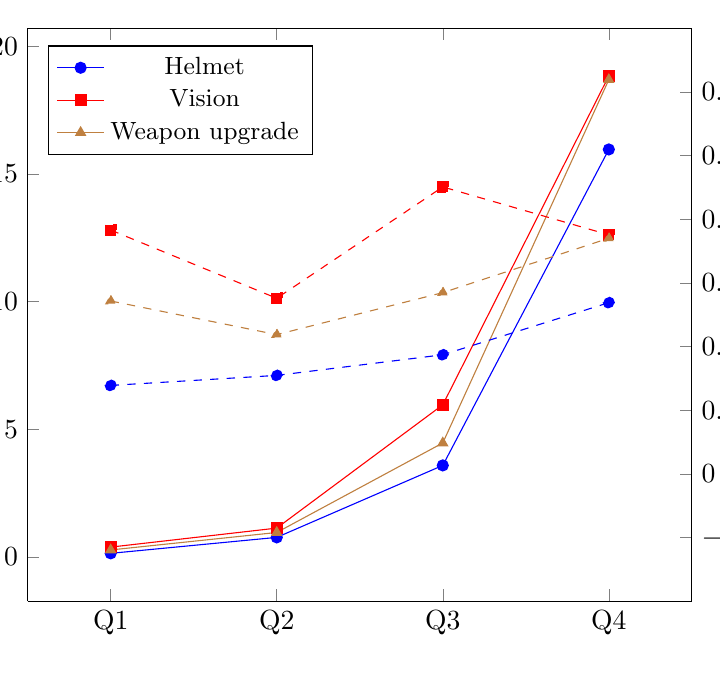
\begin{tikzpicture}[trim axis left, trim axis right]
    \pgfplotsset{set layers}
    \begin{axis}[ % avg
        scale only axis,
        ylabel=Avg. Price (solid),
        axis y line*=left,
        xmin=0.5, xmax=4.5,
        xtick=data,
        xticklabel={Q\pgfmathprintnumber{\tick}},
        legend entries={Helmet, Vision, Weapon upgrade},
        legend pos=north west,
        legend style={font=\small},
    ]
        \addplot[blue, mark=*] % Helmet
        coordinates {
            (1, 0.13879535558780817)
            (2, 0.763686440677965)
            (3, 3.582771084337348)
            (4, 15.957999999999998)
        };
        \addplot[red, mark=square*] % Vision
        coordinates {
            (1, 0.38291139240506333)
            (2, 1.1272)
            (3, 5.956296296296297)
            (4, 18.836363636363632)
        };
        \addplot[brown, mark=triangle*] % Weapon upgrade
        coordinates {
            (1, 0.27151898734177216)
            (2, 0.9558974358974357)
            (3, 4.461590909090908)
            (4, 18.690909090909088)
        };
    \end{axis}

    \begin{axis}[ % equiv
        scale only axis,
        axis x line=none,
        axis y line*=right,
        xmin=0.5, xmax=4.5,
        ymin=-0.2, ymax=0.7,
        ytick={-0.1, 0, 0.1, 0.2, 0.3, 0.4, 0.5, 0.6},
        ylabel=Equiv. Q1 Price (dashed)
    ]
        \addplot[dashed, blue, mark=*] % Helmet
        coordinates {
            (1, 0.13879535558780817)
            (2, 0.154562146892655)
            (3, 0.18697456492637202)
            (4, 0.2688148148148148)
        };
        \addplot[dashed, red, mark=square*] % Vision
        coordinates {
            (1, 0.38291139240506333)
            (2, 0.27573333333333333)
            (3, 0.4506995884773663)
            (4, 0.37542087542087527)
        };
        \addplot[dashed, brown, mark=triangle*] % Weapon upgrade
        coordinates {
            (1, 0.27151898734177216)
            (2, 0.21863247863247856)
            (3, 0.28462121212121194)
            (4, 0.37003367003366994)
        };
    \end{axis}
\end{tikzpicture}
